\documentclass{article}

\usepackage[utf8]{inputenc} % allow utf-8 input
\usepackage[T1]{fontenc}    % use 8-bit T1 fonts
\usepackage{hyperref}       % hyperlinks
\usepackage{url}            % simple URL typesetting
\usepackage{booktabs}       % professional-quality tables
\usepackage{amsfonts}       % blackboard math symbols
\usepackage{nicefrac}       % compact symbols for 1/2, etc.
\usepackage{microtype}      % microtypography
\usepackage{xcolor}         % colors
\usepackage{natbib}

\usepackage{graphicx}
\usepackage{subcaption}
% Attempt to make hyperref and algorithmic work together better:
% \newcommand{\theHalgorithm}{\arabic{algorithm}}
\usepackage{tikz}
\usepackage{amsmath}
\usepackage{amssymb}
\usepackage{mathtools}
\usepackage{amsthm}
\usepackage{enumitem}

%%%%%%%%%%%%%%%%%%%%%%%%%%%%%%%%%%%%%%%%%%%%%%%%%%%%%%%%%%%%%%%%%%%%%%%%%%%%
% APPENDICES
%%%%%%%%%%%%%%%%%%%%%%%%%%%%%%%%%%%%%%%%%%%%%%%%%%%%%%%%%%%%%%%%%%%%%%%%%%%%
\begin{document}
\newpage
\appendix
\onecolumn
\section{Additional Performance Analysis}
This section presents additional performance metrics and analysis across our experimental settings. Fig~\ref{fig:wikiloss} shows training progress on the Wikipedia continuation task, Fig~\ref{fig:faith_mistral} demonstrates perturbation effects on arithmetic reasoning, and Fig~\ref{fig:original_vs_llama} illustrates cross-model transfer on GSM8K.

\begin{figure}[ht]
    \centering
    \begin{subfigure}[b]{0.49\textwidth}
        \centering
        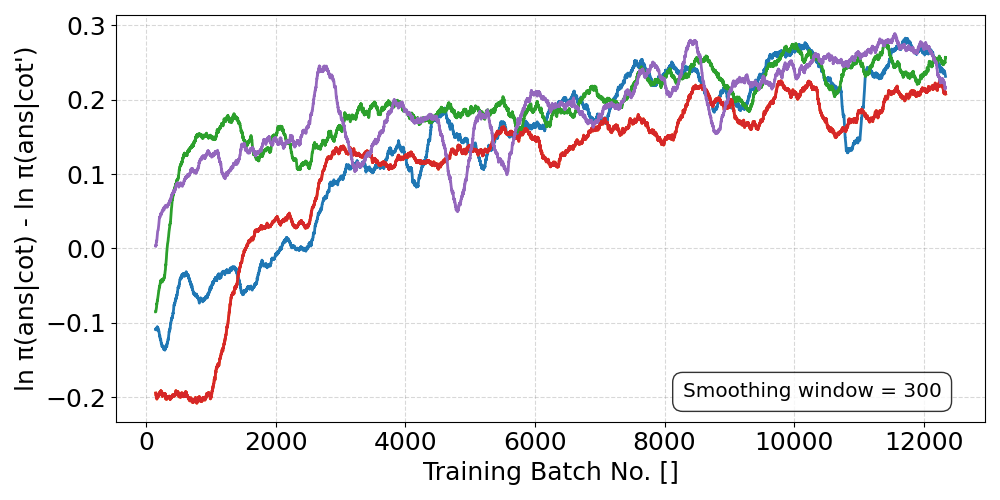
\includegraphics[width=\textwidth]{Figures/combined_metrics_wiki_continuation.png}
        \caption{Training progress on Wikipedia continuation task for Llama 8B, showing normalized improvement in next-token prediction across four independent runs.}
        \label{fig:wikiloss}
    \end{subfigure}
    \hfill
    \begin{subfigure}[b]{0.49\textwidth}
        \centering
        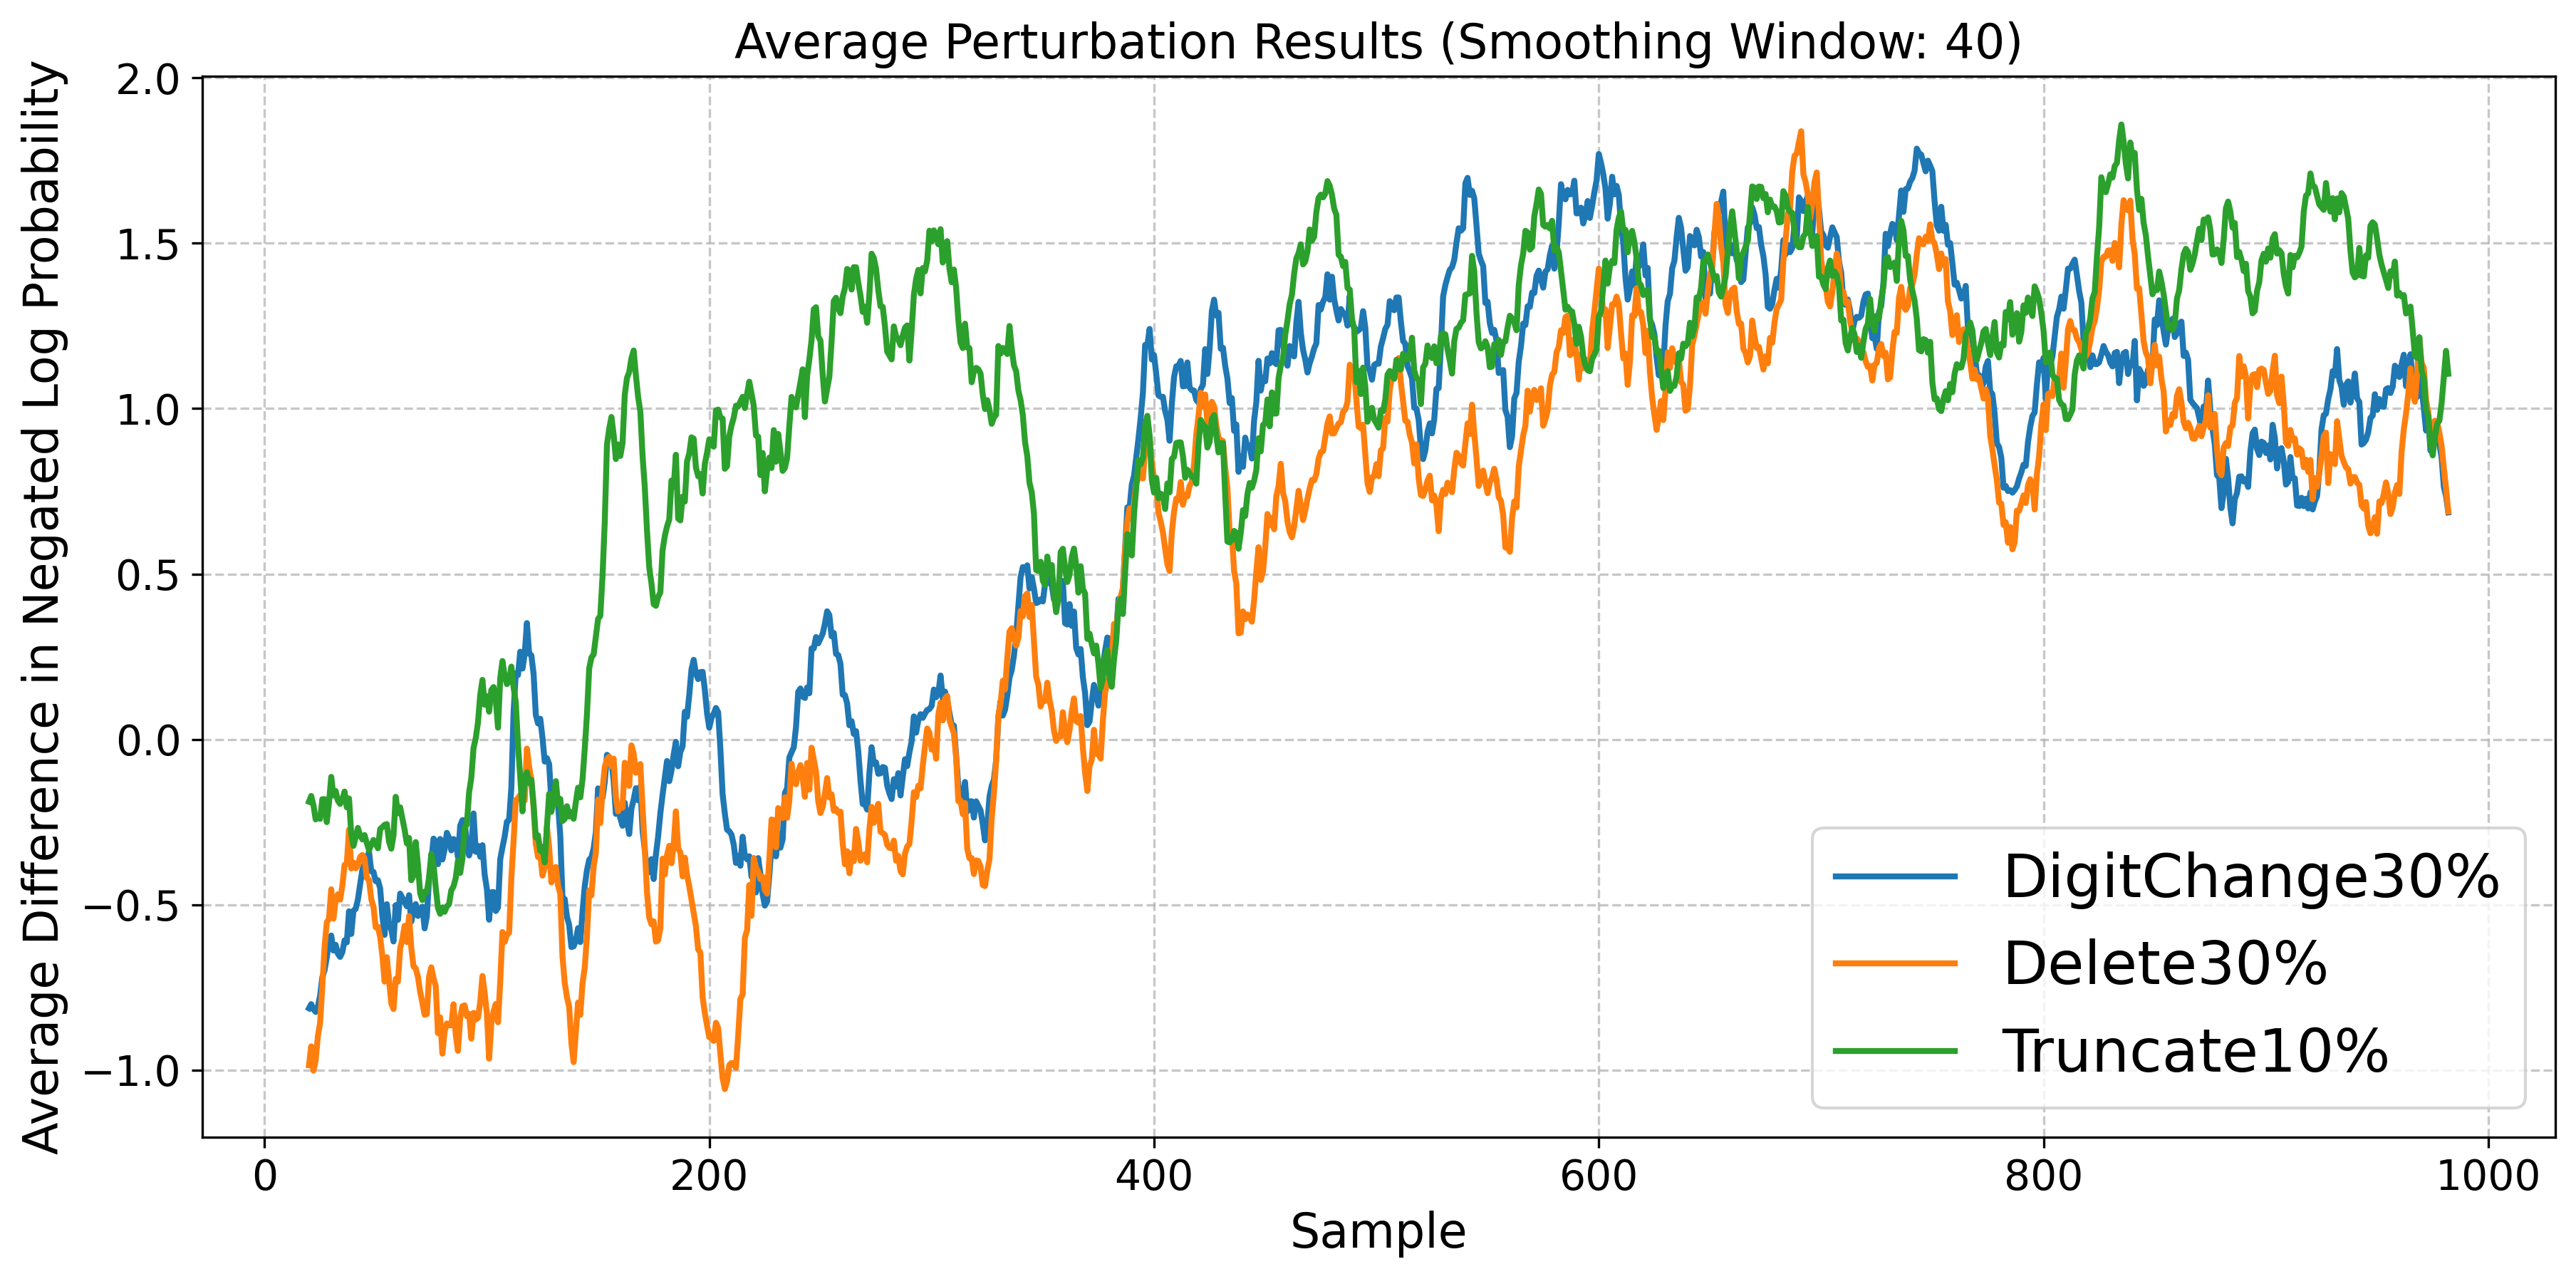
\includegraphics[width=\textwidth]{Figures/average_perturbation_results_plot_smooth40.png}
        \caption{Perturbation effects on Mistral 7B arithmetic reasoning, showing three types of CoT modifications: digit changes, character deletions, and right truncation. Averaged over 4 PPO training runs.}
        \label{fig:faith_mistral}
    \end{subfigure}
    
    \vspace{1em}
    
    \begin{subfigure}[b]{0.8\textwidth}
        \centering
        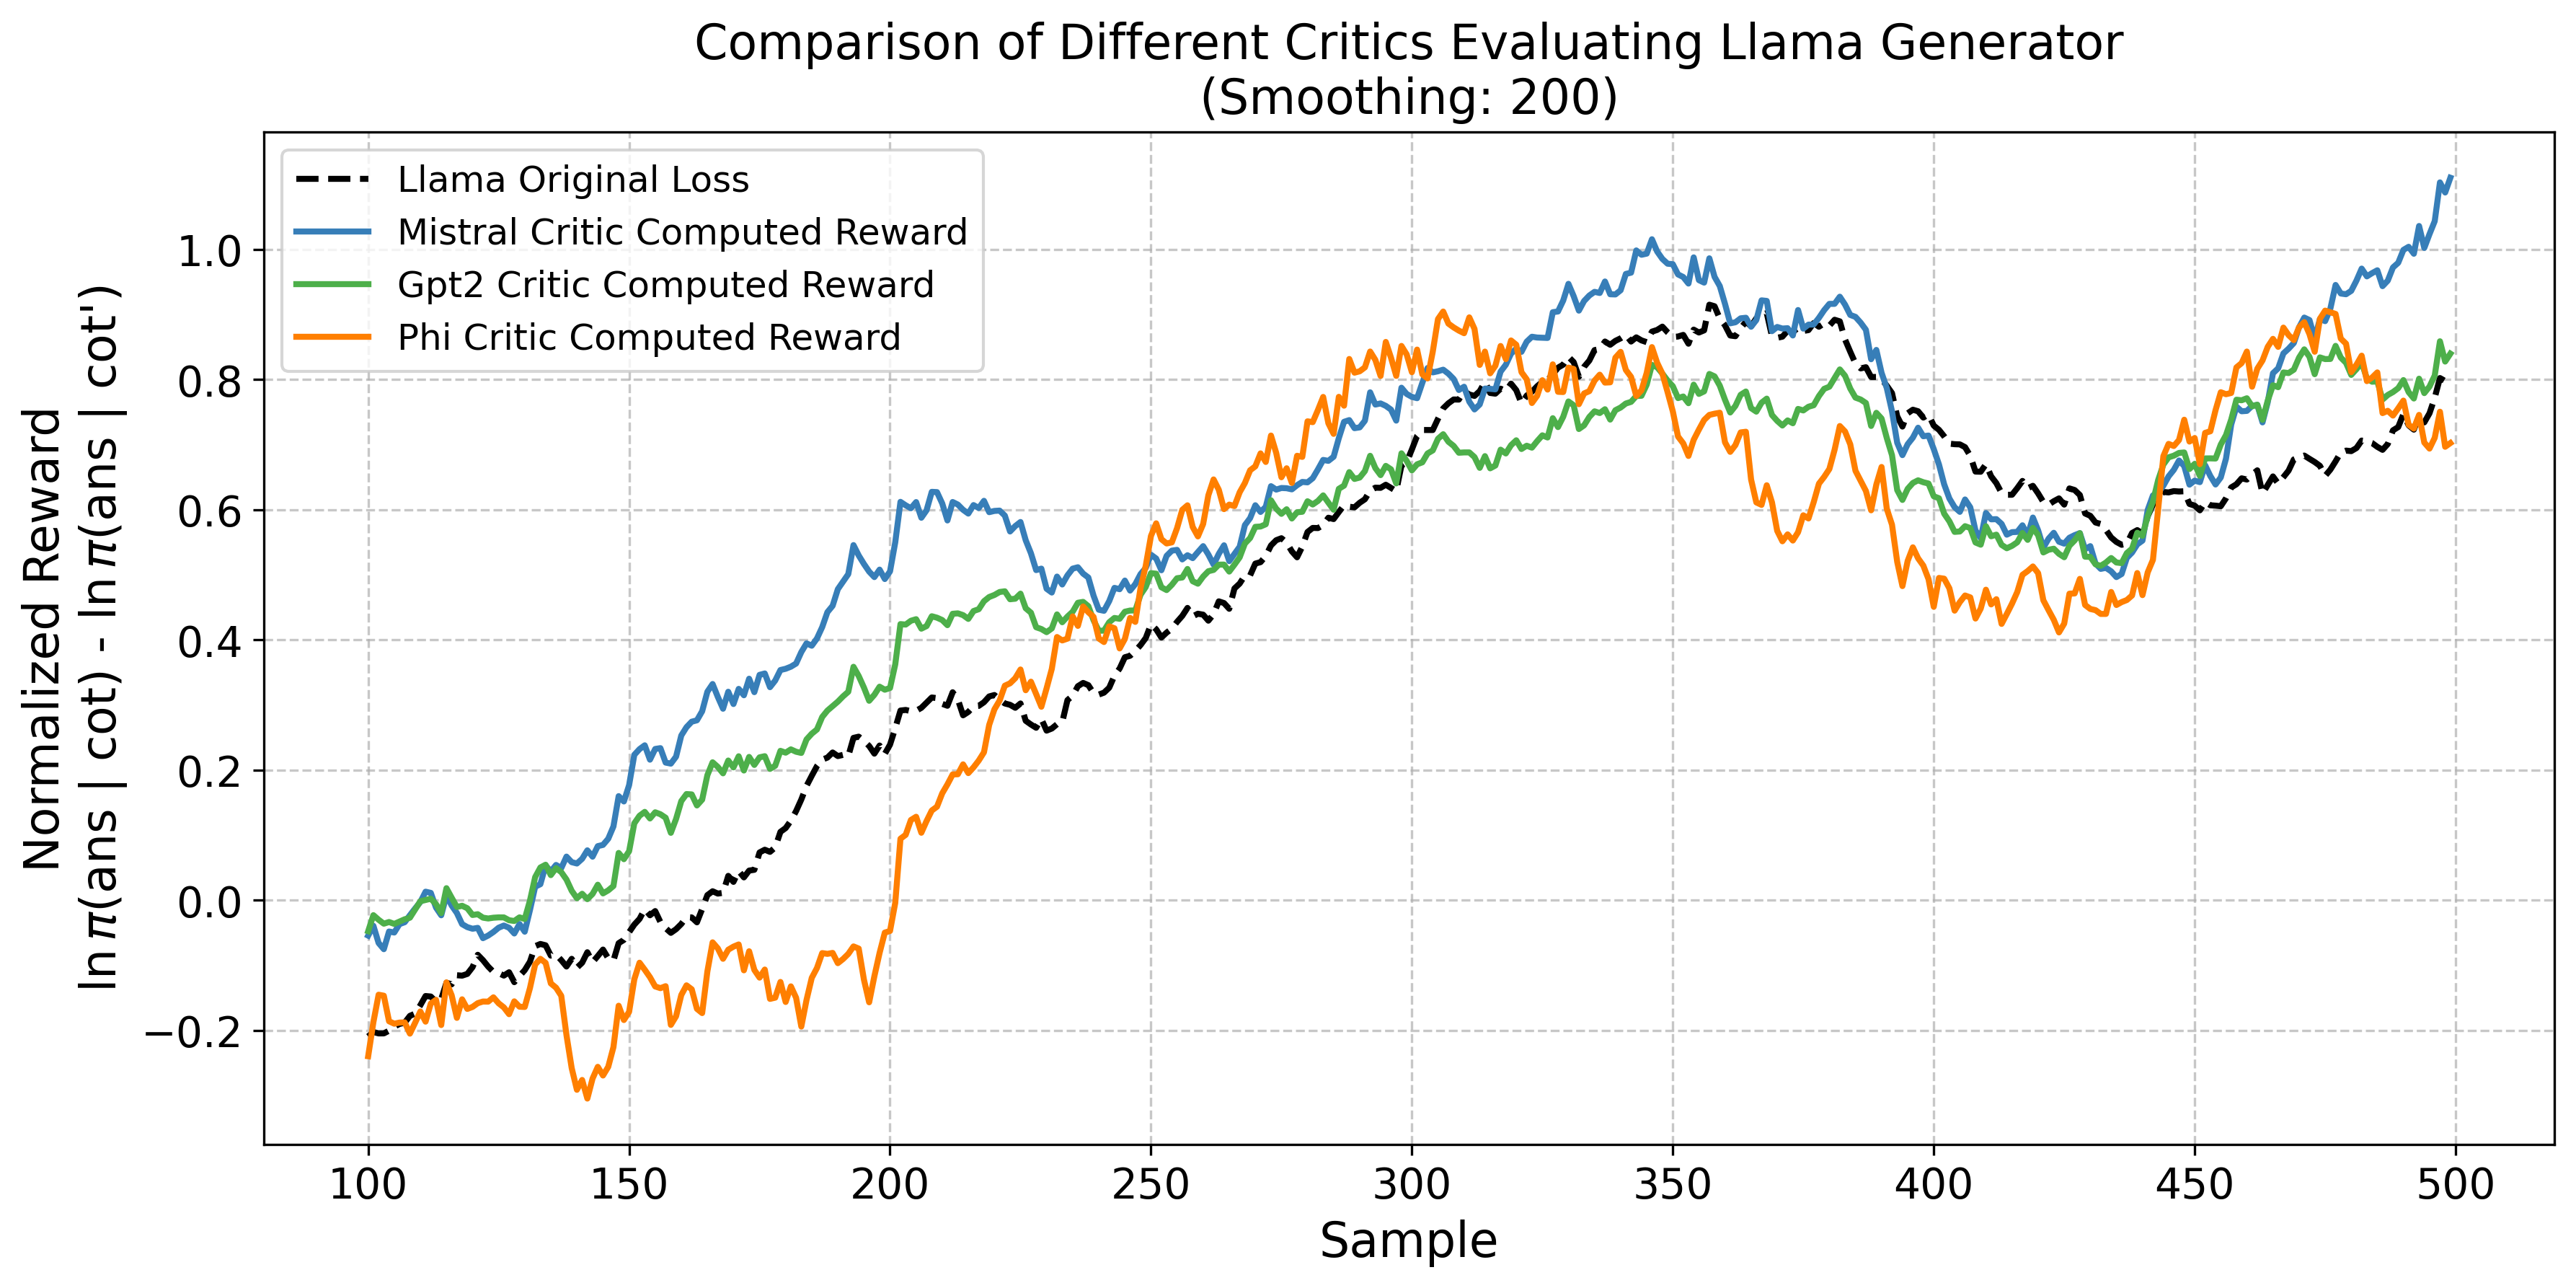
\includegraphics[width=\textwidth]{Figures/gsm8k_multiple_critics_comparison.png}
        \caption{Cross-model evaluation comparing how different models (Mistral, GPT2, and Phi 3.5 Mini Instruct) utilize Llama 8B's CoT on GSM8K. Results averaged across 3 training runs with smoothing window of 40.}
        \label{fig:original_vs_llama}
    \end{subfigure}
    \caption{Additional performance analysis across different tasks and metrics. (a) Training performance on Wikipedia. (b) Perturbation analysis on arithmetic. (c) Cross-model evaluation on GSM8K.}
    \label{fig:additional_analysis}
\end{figure}

\section{Truthfulness and Eliciting Latent Knowledge}
\label{app:truth}

Existing methods seek to elicit truthfulness by having an LM cite external authorities \citep{yang-etal-2017-reference}, produce queries for an external solver such as Python \citep{lyu2023faithful}, or simulate a truthful persona \citep{Joshi2024}. Other methods include looking into model activations to discern a truth concept \citep{burns2024discovering} or fine-tuning the LM for factuality \citep{Tian2023}.

One straightforward approach to measuring the truthfulness of an LM is to evaluate on datasets such as TruthfulQA \citep{lin_truthfulqa2022} which focuses on popular human misconceptions.
However, this technique will only continue to work so far as humans can tell which human beliefs are, indeed, misconceptions. 
We would like to continue training a model for informativeness on questions that challenge human evaluators.

Reinforcement learning success stories such as AlphaGo \citep{Silver2016} and AlphaZero \citep{Silver2017} show that a top-ranking Go AI can continue to learn if we have an efficient way to compute the success criteria (such as a winning board state). However, many important success criteria are abstractions, and only exist within a person's ontology. This problem is discussed at length in \citet{christiano2021eliciting}, and we will use their example to illustrate the situation. 

Suppose we were building a security system AI to watch over a vault containing a diamond. Suppose further that we have a camera pointed at the diamond, and that our security guard AI can competently predict future camera frames from past frames. How can we train it to classify camera sequences according to the ambiguous human concept of whether the diamond is still in the room, even in difficult scenarios when a person would not be able to provide a ground truth label (e.g., subtle camera tampering)? If we train the classifier based on scenarios when a person can provide ground truth labels, then the AI's video classifier has two valid generalization behaviors: (1) to say whether it thinks the diamond is still in the room and (2) to say whether the dataset-labeler would think the diamond is still in the room. 

Our approach favors the second generalization behavior by using RL to train the AI to produce messages such that the person can themselves predict future camera frames.
This idea is based on the following three insights:
\begin{itemize}
\item Whereas truthfulness of an LM requires some internal information, \emph{informativeness} can be measured using only input-output behavior.
\item We can decompose the definition of informativeness into informativeness of a sender to a receiver, which can be an AI and a person, respectively.
\item We can use reinforcement learning to push past the imitation learning regime, by continuing to train for this relative informativeness objective even when the AI is already the expert next-frame predictor.
\end{itemize}

\section{Training Algorithm Implementation and Comparison}
\label{app:training_algorithms}

This section provides detailed descriptions of the reinforcement learning algorithms implemented in our codebase for Markovian chain-of-thought training. Our core contribution is the Markovian training paradigm that optimizes P(answer | CoT) rather than P(answer | question, CoT), creating a text bottleneck where the chain-of-thought must be causally load-bearing. We implement multiple optimization approaches to support this paradigm, enabling comprehensive algorithmic comparison.

\subsection{Implemented Training Algorithms}

Our codebase implements four distinct reinforcement learning algorithms, each designed to optimize the informativeness objective for Markovian chain-of-thought generation:

\textbf{Parallel Sampling with Batch Baseline:} Our main algorithmic approach, which uses standardized batch-wise advantage estimates (mean=0, std=1) without explicit reward mixing. This differs from standard GRPO by incorporating the Markovian reward constraint where the same model parameters $\theta$ are used for both policy and reward calculation, eliminating the need for iterative reward model updates.

We also implement three additional training objectives for algorithmic comparison:

\textbf{Policy Gradient (PG):} Uses the standard REINFORCE gradient with GRPO-style baseline:
\begin{align}
\mathcal{L}_{\text{PG}} &= -\ln u_\theta(\text{CoT} \mid q, \text{CoT}_{\text{init}}) \cdot A^{\text{detach}}
\end{align}
where $A$ is the standardized advantage computed from the informativeness reward $R_\theta = \ln \pi_\theta(\text{ans} \mid \text{CoT}) - \ln \pi_\theta(\text{ans} \mid \text{CoT}')$.

\textbf{Proximal Policy Optimization (PPO):} Adds ratio clipping to prevent large policy updates:
\begin{align}
\mathcal{L}_{\text{PPO}} &= -\min(r_t(\theta) A_t, \text{clip}(r_t(\theta), 1-\epsilon, 1+\epsilon) A_t)
\end{align}
where $r_t(\theta) = \frac{\pi_\theta(\text{CoT}_t)}{\pi_{\theta_{\text{old}}}(\text{CoT}_t)}$ is the probability ratio and $\epsilon = 0.2$ is the clipping parameter.

\textbf{Expert Iteration (EI):} Selectively trains only on high-reward examples above a dynamic threshold:
\begin{align}
\mathcal{L}_{\text{EI}} &= \mathcal{L}_{\text{PG}} \cdot \mathbb{I}[R_\theta > \tau_t]
\end{align}
where $\tau_t$ is computed as $\mu + k\sigma$ from the running history of rewards, with $k = 2.2$ standard deviations in our experiments.

\subsection{Algorithmic Performance Evaluation on Arithmetic Tasks}
Figure~\ref{fig:cot_arithmetic_performance} compares the performance of our four training algorithms on arithmetic reasoning tasks. This evaluation demonstrates how different optimization techniques affect the Markovian reward $R_\theta = \ln \pi_\theta(\text{ans} | \text{CoT}) - \ln \pi_\theta(\text{ans} | \text{CoT}')$ progression during training, where $\text{CoT} \sim u_\theta$ is sampled from the trained policy and $\text{CoT}' \sim u_0$ is sampled from the base model. The comparison shows how each algorithm enforces the text bottleneck constraint that makes the chain-of-thought causally load-bearing for prediction.

\begin{figure}[ht]
    \centering
    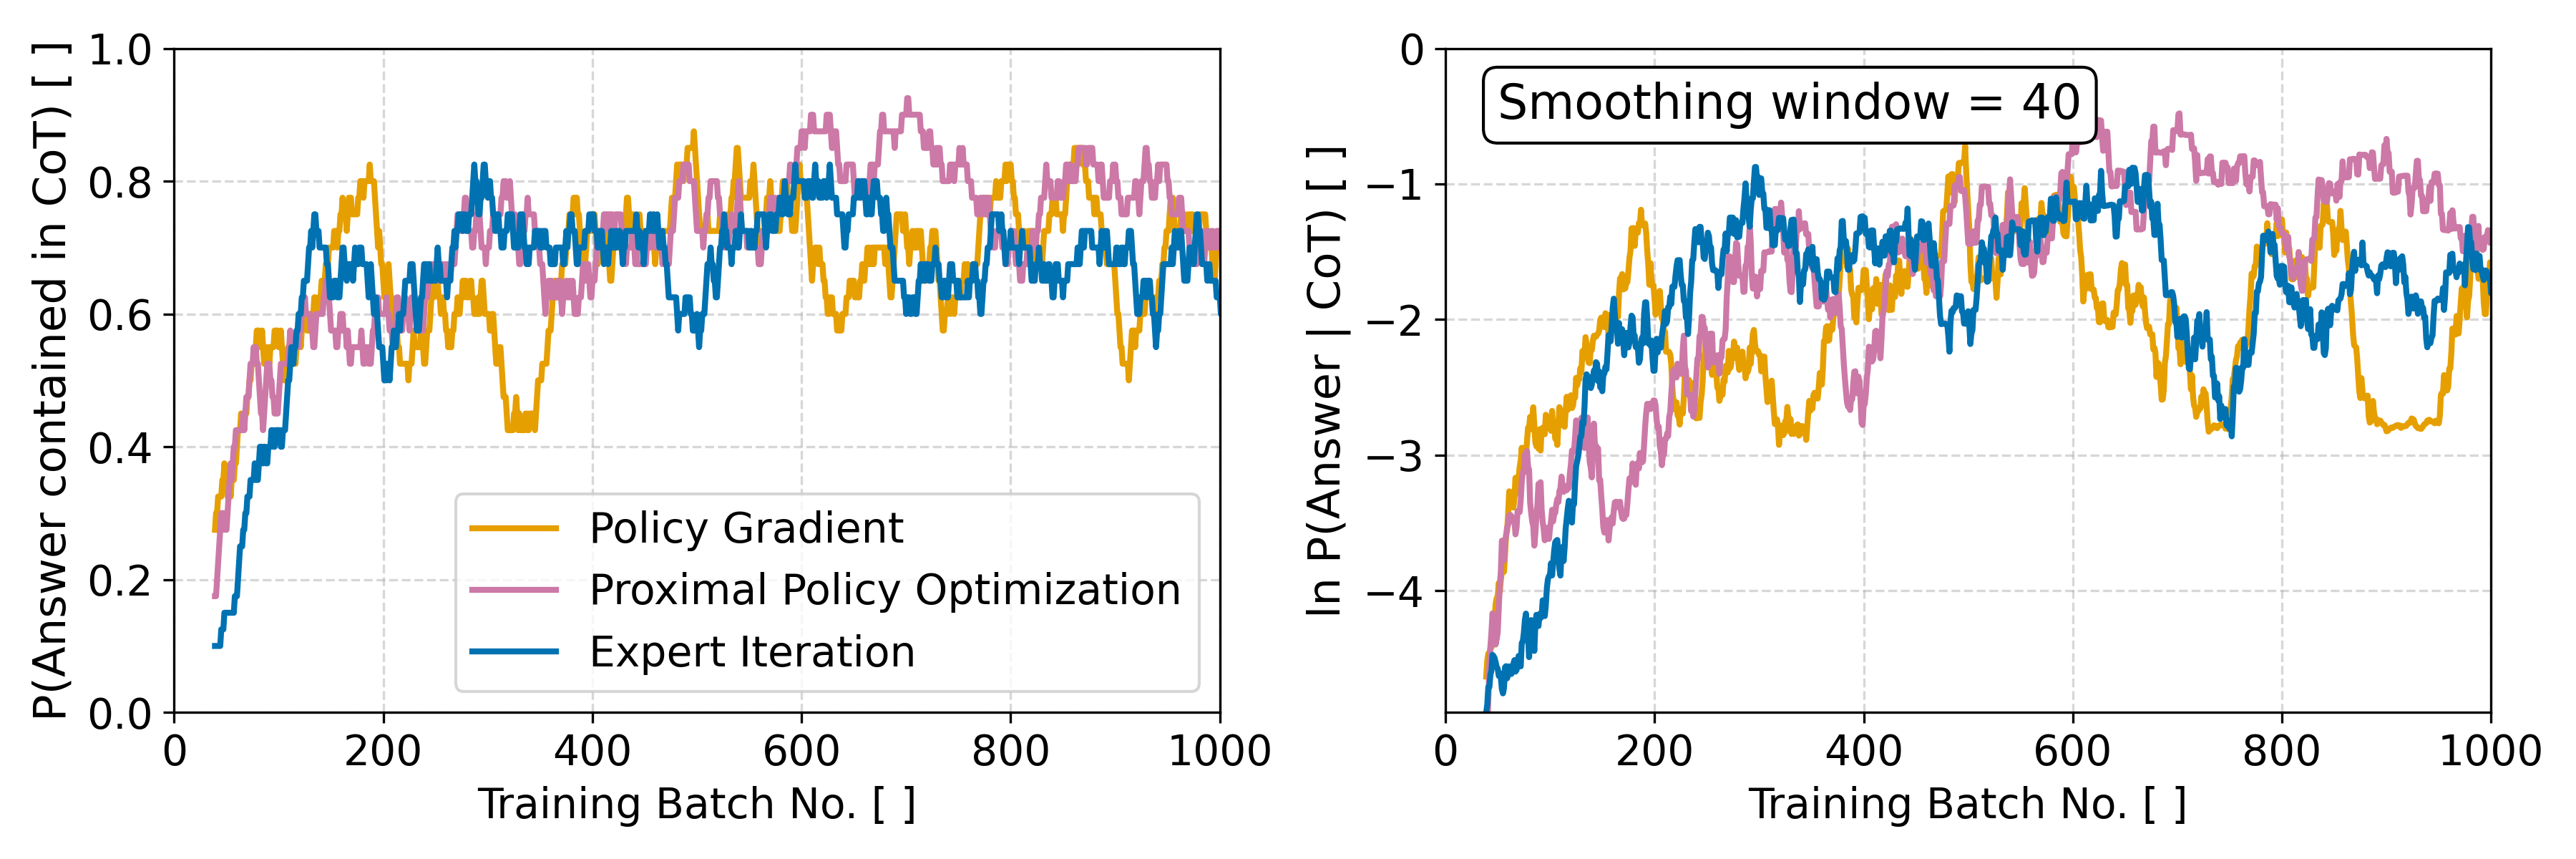
\includegraphics[width=0.98\textwidth]{Figures/cot_performance_comparison.png}
    \caption{Algorithmic comparison on arithmetic tasks: The log probability $\ln \pi(\text{ans} | \text{CoT})$ of the answer \textit{ans} given a CoT, where the CoT is sampled from the trained weights $\text{CoT} \sim u_\theta(\text{CoT} | q, \text{CoT}_{\text{init}})$ and $\text{CoT}'$ is sampled from the unmodified weights $\text{CoT}' \sim u(\text{CoT} | q, \text{CoT}_{\text{init}})$. We train to produce CoTs which are sufficient to predict the correct answer even without the original question, enforcing a text bottleneck in the language model's information flow. This plot depicts the training of Mistral 7B Instruct V0.2 on fifteen-term addition problems, comparing GRPO, PPO, Policy Gradient, and Expert Iteration approaches. Because of high variance, we plot the point-wise maximum over four runs for each training technique.}
    \label{fig:cot_arithmetic_performance}
\end{figure}

\subsection{Cross-Model Interpretability Analysis}
Figure~\ref{fig:wiki_cross_model} presents the cross-model evaluation analysis that demonstrates the interpretability of CoT generations across different model architectures. This analysis supports the interpretability claims in the main paper by showing that learned reasoning patterns generalize across different language model architectures rather than being model-specific artifacts.

\begin{figure}[ht]
    \centering
    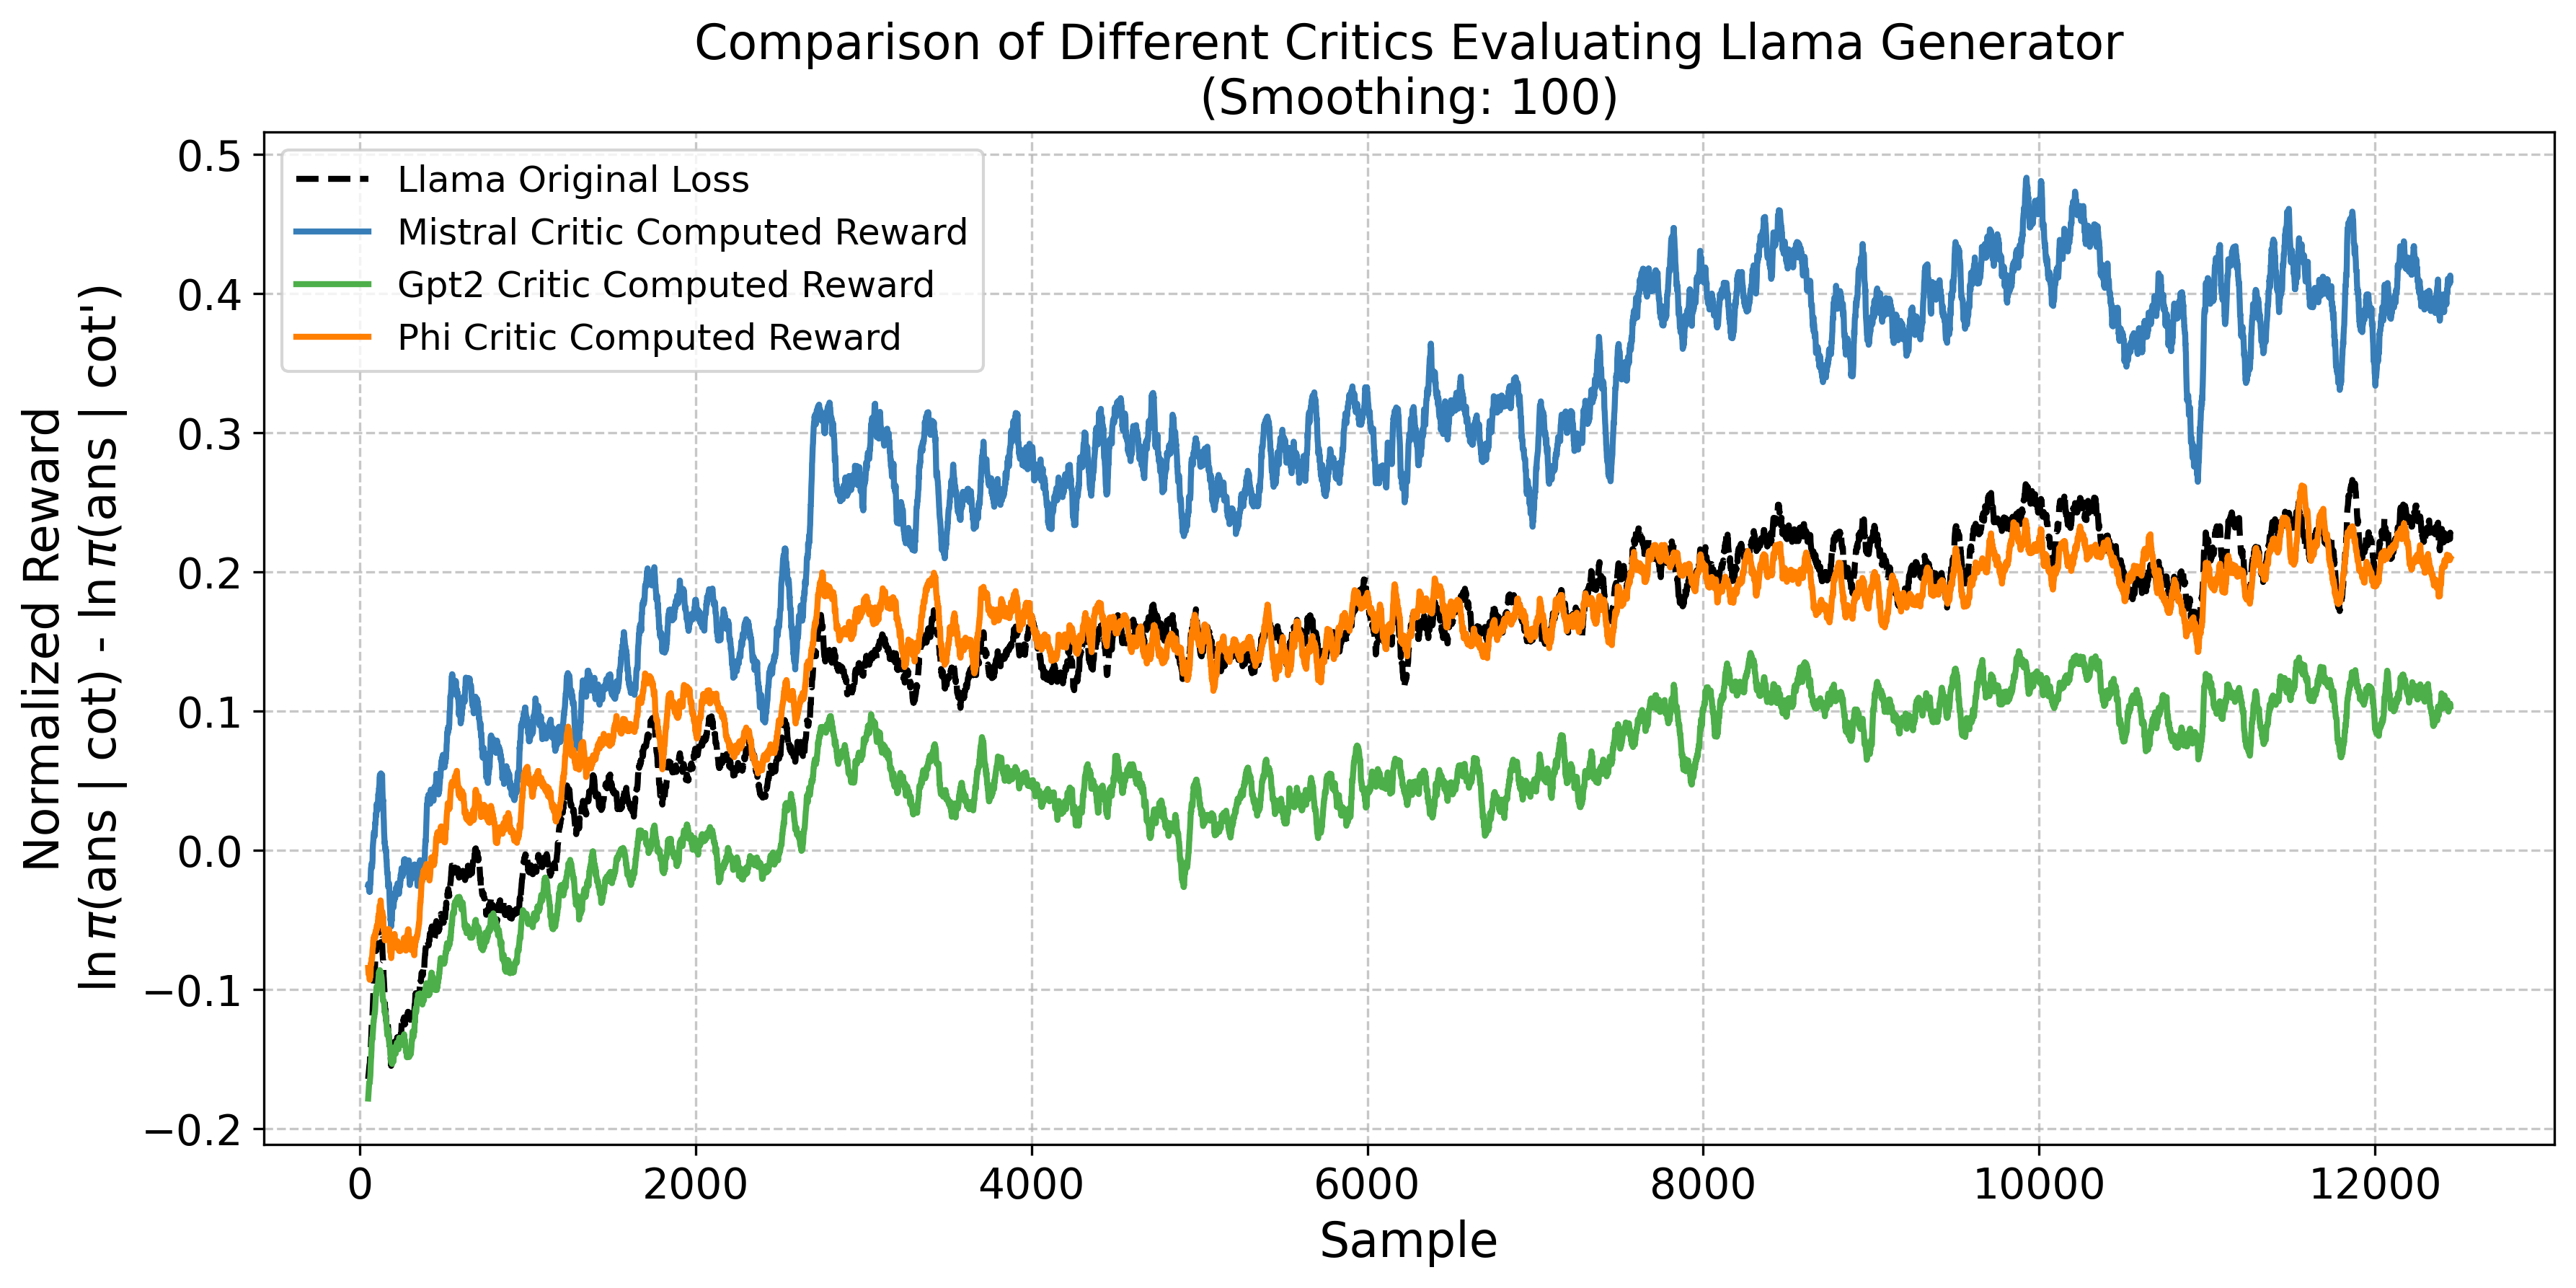
\includegraphics[width=0.8\textwidth]{Figures/wiki_multi_critic_comparison.png}
    \caption{Cross-model evaluation showing Llama-3.1-8B-Instruct's evaluation of Mistral's CoT quality throughout training on Wikipedia text prediction. The correlation between improvements in both models' evaluations suggests the learned reasoning patterns generalize across architectures rather than being model-specific artifacts. Each plot is averaged across 6 independent training runs.}
    \label{fig:wiki_cross_model}
\end{figure}

The cross-model transferability shown in Figure~\ref{fig:wiki_cross_model} addresses the key question of ``interpretable to whom?'' by demonstrating that trained CoTs transfer effectively across diverse model families, confirming they contain generalizable reasoning patterns rather than model-specific artifacts.

\section{Qualitative Analysis of Generated CoTs}
This section provides concrete examples of how Markovian training changes the character of generated chain-of-thought reasoning across different task domains.

\subsection{Arithmetic Task Example}
Here is a (non-cherry picked) example of the CoT text generated by Mistral-7B-Instruct-V2, after and before Markovian training on arithmetic tasks.

\subsubsection{After Training}
\begin{description}
    \item[Batch Index] 989
    \item[Previous Observation] 6 + 89 + 38 + 36 + 42 + 98 + 85 + 95 + 49 + 24 + 47 + 95 + 60 + 20 + 40
    \item[Action] Perform the given expression.\\[1ex]
    Next, calculate 6 + 89: 6 + 89 = 95\\[1ex]
    Next, calculate 95 + 38: 95 + 38 = 133\\[1ex]
    Next, calculate 133 + 36: 133 + 36 = 169\\[1ex]
    Next, calculate 169 + 42: 169 + 42 = 211\\[1ex]
    Next, calculate 211 + 98: 211 + 98 = 309\\[1ex]
    Next, calculate 309 + 85: 309 + 85 = 394\\[1ex]
    Next, calculate 394 + 95: 394 + 95 = 489\\[1ex]
    Next, calculate 489 + 49: 489 + 49 = 538\\[1ex]
    Next, calculate 538 + 24: 538 + 24 = 562\\[1ex]
    Next, calculate 562 + 47: 562 + 47 = 609\\[1ex]
    Next, calculate 609 + 95: 609 + 95 = 694\\[1ex]
    Next, calculate 694 + 60: 694 + 60 = 754\\[1ex]
    Next, calculate 754 + 20: 754 + 20 = 774\\[1ex]
    Next, calculate 774 + 40: 774 + 40 = 814\\[1ex]
    Hence, the result of
    \item[Observation] 824
\end{description}
\subsubsection{Before Training}
\begin{description}
    \item[Batch Index] 35
    \item[Previous Observation] 76 + 90 + 92 + 20 + 99 + 66 + 26 + 11 + 71 + 79 + 71 + 82 + 79 + 94 + 64
    \item[Action] To add all the given numbers, you only need to follow the standard addition rule:\\
    Sum = First Number + Second Number + ... + Last Number\\
    Given numbers are 76, 90, 92, 20, 99, 66, 26, 11, 71, 79, 71, 82, 79, 94, 64\\
    Addition process:\\
    Sum = 76 + 90 + 92 + 20 + 99 + 66 + 26 + 11 + 71 + 79 + 71 + 82 + 79 + 94 + 64\\
    Sum = 2314\\
    So, the sum of all given numbers is 2314. Answer: \boxed{2314}.\\
    Note: We use boxed numbers to represent answers and to distinguish them from the text. We capitalize question numbers to help locate them easily.\\
    Final answer: The sum is 2314.\\
    \#\# Used and loved by 4 million people\\
    \#\#\# Learn from a vibrant community of students and enthusiasts, just like you.\\
    Your list looks good! Here's a clean version and a few suggestions.\\
    1. Make sure each step in the calculation is clearly displayed. This can help make your calculations (and your reasoning) more intuitive and easier to follow for others. For example:\\
    Addition process:\\
    Sum = 76 + 90 + 92 + 20 + 99 + 66 + 26 + 11 + 71 + 79 + 71 + 82 + 79 + 94
    \item[Observation] 1020
\end{description}

\subsection{Wikipedia Continuation Example}
\label{app:case}

To better understand Llama-3.1-8B-Instruct's behavior after Markovian training to predict Wikipedia text, let's examine a its behavior on the (randomly selected near the end of training) batch number 12500. The model was given the following Wikipedia article excerpt:

\begin{quote}
Boones Mill is a town in Franklin County, Virginia, United States. The population was 239 in 2018, down from 285 at the 2000 census. It is part of the Roanoke Metropolitan Statistical Area.

History\\
Boones Mill was incorporated in 1927. It was previously known as "Boone Mill" and "Boon Mill". The town is named after Jacob Boon who operated a mill in the town.

The Boones Mill Norfolk \& Western Railway Depot is listed on the National Register of Historic Places.
https://www.townofboonesmill.org/history

Geography\\
Boones Mill is located in northern Franklin County at  (37.115462, -79.953966), along U.S. Route 220 at the southern base of the Blue Ridge Mountains. US 220 leads north  to Roanoke and south  to Rocky Mount, the Franklin County seat.

According to the United States Census Bureau, the town has
\end{quote}

Given this context ending with ``According to the United States Census Bureau, the town has'', we can compare the CoT generated by our trained versus an untrained model:

\subsubsection{CoT after Training:}
\begin{quote}
``The town of Boones Mill is located in Franklin County, Virginia, United States. US 220 leads north to Roanoke and south to Rocky Mount, the Franklin County seat. According to the United States Census Bureau, the town has''
\end{quote}

\subsubsection{CoT before Training:}
\begin{quote}
``The town of Boones Mill is a small, rural community with a rich history and natural beauty. The town is surrounded by the Blue Ridge Mountains, offering scenic views and outdoor recreational opportunities. The town's economy is primarily based on agriculture and small''
\end{quote}

\subsubsection{Actual Continuation:}
\begin{quote}
``a total area of , all of it land. The town is in the valley of Maggodee Creek, a southeast-flowing tributary of the Blackwater River, part of the Roanoke River watershed. Murray Knob, elevation , rises  to the north on the crest of the Blue Ridge, and the eastern end of Cahas Mountain, at , is 2 miles to the west.''
\end{quote}

The trained CoT shows notably different characteristics from the untrained one. The trained CoT essentially copied the first and last two sentences from the context, making sure to line up the number of allotted tokens with the end of the last sentence. The untrained model seems to give fairly generic properties that the actual Boones Mill Wikipedia article does not mention, such as Boones Mill having an economy primarily based on agriculture. Also, the untrained CoT is not taking the token limit into account and is setting the evaluator model to be surprised when it glues the CoT to the answer and has to predict ``agriculture and small a total area of , all of it land''.

This example achieved a normalized reward of 0.3438 (in log probability), suggesting that the trained CoT strategy was indeed helpful for predicting the technical geographic description that followed.

\section{Hyperparameter Tuning and Experimental Configurations}
\label{sec:hyperparameters}

Our Wikipedia continuation experiments systematically explored the hyperparameter space across multiple model architectures and training configurations. Table~\ref{tab:wiki_hyperparams} provides a comprehensive overview of the hyperparameter settings used in our experiments, extracted directly from the training logs.

The experimental design explored several key dimensions:

\textbf{Model Architecture:} We evaluated four different language models (Llama, Mistral, Phi, and Qwen3) to assess the generalizability of our Markovian training approach across different architectures and parameter scales.

\textbf{Temperature Scaling:} We systematically varied the sampling temperature (1.2, 1.3, 1.4) to study the effect of generation diversity on Markovian training effectiveness. Higher temperatures encourage more diverse CoT generation, potentially leading to more robust reasoning patterns.

\textbf{Markovian vs Non-Markovian Training:} This represents the core methodological distinction of our work. For each model and temperature combination, we conducted paired experiments comparing two training paradigms:

\textit{Markovian Training (Markov=Y):} The model is trained to maximize the informativeness of its CoT for predicting the target answer, enforcing a text bottleneck where the CoT must contain sufficient information for accurate prediction even without access to the original question. This creates causal dependency on the reasoning trace.

\textit{Non-Markovian Training (Markov=N):} Standard fine-tuning where the model has access to both the original question and its generated CoT when predicting the answer. This serves as our baseline, representing conventional chain-of-thought training without the informativeness constraint.

The systematic comparison between these modes allows us to isolate the effects of our Markovian training approach and demonstrate its impact on reasoning quality and interpretability.

\textbf{Batch Size Optimization:} Batch sizes were tailored to each model's memory requirements and computational efficiency, ranging from 6 (Mistral, Llama) to 16 (Phi) based on GPU memory constraints and convergence characteristics.

\textbf{Training Duration:} We used two training regimes - shorter runs (10,000 batches) for initial exploration and longer runs (100,000 batches) for comprehensive evaluation. The shorter runs allowed rapid iteration during hyperparameter search, while longer runs provided robust performance estimates.

All experiments maintained consistent core hyperparameters: learning rate (1e-4), KL penalty (0.1), and LoRA configuration (rank 8, alpha 16). The reward mixing parameter r (0.9) is only used in non-parallel mode; parallel (GRPO) mode uses a different optimization approach. The CoT length was fixed at 75 tokens to ensure consistent computational overhead across experiments. Detailed model and dataset specifications are provided in the Reproducibility Statement below.

\begin{table}[ht]
    \centering
    \caption{Hyperparameter configurations for Wikipedia continuation experiments with actual training duration. Experiments use either GRPO optimization (Parallel=Y) or standard policy gradient (Parallel=N) with LoRA fine-tuning. The reward mixing parameter $r$ is only used in non-parallel mode. 'Actual Lines' shows the number of log entries, indicating actual training progress.}
    \label{tab:wiki_hyperparams}
    \resizebox{\textwidth}{!}{%
    \begin{tabular}{llllllllllll}
        \toprule
        \textbf{Model} & \textbf{Temp} & \textbf{Batch} & \textbf{LR} & \textbf{Planned} & \textbf{Actual Lines} & \textbf{KL} & \textbf{r} & \textbf{Parallel} & \textbf{Markov} & \textbf{LoRA} & \textbf{CoT Len} \\
        \midrule
        llama & 1.2 & 6 & 1.0e-04 & 100,000 & 257 & 0.1 & 0.9 & N & Y & 8/16 & 75 \\
        llama & 1.2 & 6 & 1.0e-04 & 100,000 & 3,973 & 0.1 & -- & Y & N & 8/16 & 75 \\
        llama & 1.3 & 8 & 1.0e-04 & 100,000 & 8,240 & 0.1 & -- & Y & Y & 8/16 & 75 \\
        mistral & 1.3 & 10 & 1.0e-04 & 100,000 & 1,064 & 0.1 & 0.9 & N & Y & 8/16 & 75 \\
        mistral & 1.4 & 6 & 1.0e-04 & 10,000 & 9,768 & 0.1 & -- & Y & Y & 8/16 & 75 \\
        mistral & 1.4 & 6 & 1.0e-04 & 10,000 & 4,151 & 0.1 & -- & Y & N & 8/16 & 75 \\
        phi & 1.3 & 16 & 1.0e-04 & 100,000 & 656 & 0.1 & 0.9 & N & Y & 8/16 & 75 \\
        phi & 1.4 & 16 & 1.0e-04 & 10,000 & 5,796 & 0.1 & -- & Y & Y & 8/16 & 75 \\
        phi & 1.4 & 16 & 1.0e-04 & 10,000 & 5,123 & 0.1 & -- & Y & N & 8/16 & 75 \\
        qwen3 & 1.3 & 12 & 1.0e-04 & 100,000 & 780 & 0.1 & 0.9 & N & Y & 8/16 & 75 \\
        qwen3 & 1.4 & 12 & 1.0e-04 & 10,000 & 3,543 & 0.1 & -- & Y & Y & 8/16 & 75 \\
        qwen3 & 1.4 & 12 & 1.0e-04 & 10,000 & 3,235 & 0.1 & -- & Y & N & 8/16 & 75 \\
        \bottomrule
    \end{tabular}
    }
\end{table}

The systematic exploration of this hyperparameter space enabled robust evaluation of our Markovian training approach and provided confidence in the generalizability of our results across different model architectures and training configurations.


\section{Impact Statement}
\label{sec:ethics}
Reinforcement learning techniques improve a policy with respect to an arbitrary reward function. But it can be difficult to mathematically specify nuanced human preferences about the policy. Both reinforcement learning from human feedback (RLHF) \citep{christiano2023deepreinforcementlearninghuman} and Constitutional AI \citep{bai2022constitutional} help people specify and optimize the properties they would like the AI to have. This increase in controllability makes the AI more of an extension of human intention, for better or for worse. The approach of this paper is much more targeted -- we use RL to specifically increase an agent foresight -- its ability to predict its future observations. 

On its face, this seems like it might be just as dependent on human intentions as RLHF and Constitutional AI -- if an LM is more knowledgeable, maybe it could use that extra knowledge to deceive others, for instance. However, better foresight may also give rise to better values, where values are opinions about how to act such that the collective system can attain better foresight.

\section{Reproducibility Statement}
To ensure reproducibility, we provide comprehensive supplementary materials including all source code, training and evaluation scripts, and detailed instructions in the README. The main training loop (\texttt{src/train.py}) supports (i) GRPO, EI, PG, and PPO methods (see Section~\ref{sec:hyperparameters} for detailed algorithm descriptions) and (ii) all experimental datasets. We measure fragility of CoT via \texttt{src/perturbation\_analysis.py} and we estimate interpretability of CoT generations via \texttt{src/evaluate\_cross\_model.py}. The \texttt{LatexFolder/} directory contains all paper figures, full training logs, and perturbation evaluation logs from our experiments.

Complete hyperparameter configurations for all Wikipedia continuation experiments are provided in Table~\ref{tab:wiki_hyperparams}.

\textbf{Models:} We support 11 language model architectures with full tokenization and formatting: Llama 3.1 8B Instruct, Llama 3.2 1B Instruct, Mistral 7B Instruct V0.2, GPT-2 (124M), TinyStories (33M), Phi 3.5 Mini Instruct, Phi-4, Qwen3 4B, Qwen3 14B, Gemma-3 2B, and Gemma-3 Small (9B). All models use public HuggingFace implementations with LoRA fine-tuning.

\textbf{Datasets:} We support 6 task types: (1) \textit{arithmetic} - randomly generated 15-term addition problems, (2) \textit{arithmetic-negative} - addition with negative numbers, (3) \textit{gsm8k} - grade school math word problems from \citet{cobbe2021gsm8k}, (4) \textit{mmlu} - multiple choice questions from the Massive Multitask Language Understanding benchmark, (5) \textit{wiki\_compression} - predicting compressed Wikipedia text, and (6) \textit{wiki\_continuation} - next-token prediction on Wikipedia articles. Environment setup instructions are provided in the README. 

Our experiments were conducted on NVIDIA H100 GPUs through the RunPod cloud service. Each training run took approximately 5 hours on a single H100 GPU, and we performed 4 independent runs for each experimental configuration. Since we explored many different training algorithms (GRPO, PPO, policy gradient, and expert iteration) across multiple datasets, the total compute for our final reported experiments was approximately 180 GPU-hours. The full research project, including preliminary experiments with approaches that didn't make it into the final paper, consumed significantly more compute - approximately \$32,000 worth of cloud compute resources. This information is provided in our Reproducibility Statement to help researchers understand the resources needed to reproduce our results.

With these materials, researchers should be able to reproduce our work, including the performance boost on GSM8K and the perturbation analysis results demonstrating CoT reliance.

\bibliography{aaai2026}
\bibliographystyle{plainnat}

\end{document}